\documentclass[25pt, a0paper, portrait]{tikzposter}

% =========================
% Poster metadata
% =========================
\title{CLIP: Contrastive Language--Image Pretraining}
\author{DEGENEVE Hugo, KAPOTOS Fotios}
\date{}
\institute{CentraleSupélec}

\usepackage{amsmath}

\begin{document}
\maketitle

% =========================================================
% INTRODUCTION
% What is CLIP? Why it matters? Core idea.
% =========================================================
\block{Introduction}{
    \textbf{What is CLIP?}
CLIP (Contrastive Language--Image Pretraining) learns a \textbf{shared embedding space}
for images and natural language using large-scale image--text pairs.

\textbf{Training signal.}
Instead of labeled classes, supervision comes from \textbf{natural language captions}
collected at web scale.

\textbf{Paradigm shift.}
Traditional vision models learn
\[
\text{image} \rightarrow \text{fixed label set}.
\]
CLIP learns
\[
\text{image} \leftrightarrow \text{text},
\]
enabling \textbf{open-vocabulary} recognition.

\textbf{Core idea.}
Matched image--text pairs are pulled together in the embedding space,
while mismatched pairs are pushed apart using a contrastive objective.

}

% =========================================================
% TRAINING SETUP
% How is CLIP trained and on what data?
% =========================================================
\begin{columns}

    \column{0.6}
    \block{Training Objective}{
        \textbf{Learning objective.}
CLIP is trained using a \textbf{contrastive learning} objective
that aligns images and text in a shared embedding space.

\textbf{Batch-wise training.}
Given a batch of \(N\) image--text pairs:
\begin{itemize}
    \item each image is encoded independently,
    \item each text caption is encoded independently,
    \item all \(N \times N\) similarities are computed.
\end{itemize}

\textbf{Optimization goal.}
\begin{itemize}
    \item matching image--text pairs $\rightarrow$ high similarity,
    \item mismatched pairs $\rightarrow$ low similarity.
\end{itemize}

\textbf{Key property.}
The objective is symmetric (image$\leftrightarrow$text)
and uses other samples in the batch as \textbf{implicit negatives},
making it scalable to very large datasets.

    }

    \column{0.4}
    \block{Dataset}{
        CLIP is trained on a large-scale dataset called \textbf{WebImageText (WIT)}.

\vspace{0.6em}
Key properties:
\begin{itemize}
    \item 400 million image--text pairs,
    \item collected from publicly available web data,
    \item no manual annotation or fixed label set,
    \item extremely broad semantic coverage.
\end{itemize}

\vspace{0.6em}
This scale enables CLIP to learn visual concepts aligned with natural language,
rather than a predefined taxonomy of classes.

    }

\end{columns}

% =========================================================
% SYSTEM OVERVIEW (EARLY VISUAL ANCHOR)
% =========================================================
\begin{columns}

    \column{0.7}
    \block{CLIP Training and Inference Pipeline}{
        \begin{tikzfigure}
            \centering
            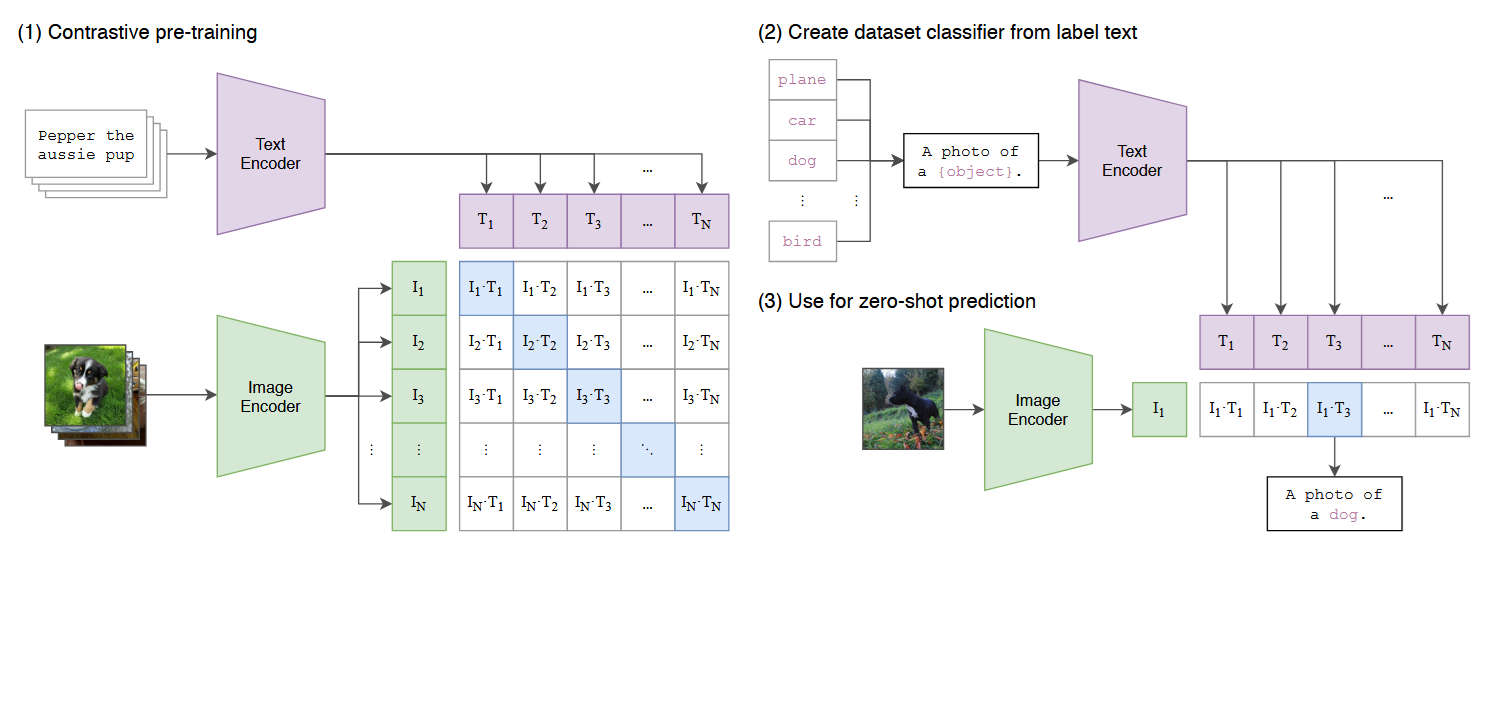
\includegraphics[width=\linewidth]{figures/clip_pipeline.png}
        \end{tikzfigure}
    }

    \column{0.3}
    \block{CLIP Training Details}{
        \textbf{Encoders.}
\begin{itemize}
    \item Image encoder \textbf{CNN or Vision Transformer}
    \item Text encoder \textbf{Transformer}
    \item \textbf{No cross-attention}: modalities interact only through the loss
\end{itemize}

\textbf{Training loss (contrastive).}
\begin{itemize}
    \item For a batch of \(N\) image--text pairs, compute all \(N \times N\) similarities
    \item Image-to-text loss:
    \[
    \mathcal{L}_{\text{img}\rightarrow\text{text}}
    = - \frac{1}{N} \sum_{i=1}^N
    \log \frac{\exp(s_{ii}/\tau)}{\sum_{j=1}^N \exp(s_{ij}/\tau)}
    \]
    \item Text-to-image loss defined symmetrically
    \item Final loss:
    \[
    \mathcal{L}
    = \tfrac{1}{2}
    \left(
    \mathcal{L}_{\text{img}\rightarrow\text{text}}
    +
    \mathcal{L}_{\text{text}\rightarrow\text{img}}
    \right)
    \]
\end{itemize}

\textbf{Inference (zero-shot).}
\begin{itemize}
    \item Embed text prompts once
    \item Classify images by \textbf{nearest-neighbor retrieval}
    \item No task-specific training required
\end{itemize}

    }

\end{columns}

%
% INFERENCE & PERFORMANCE (3-COLUMN COMPRESSION)
% =========================================================
\begin{columns}

    \column{0.33}
    \block{Zero-Shot Classification}{
        \textbf{Zero-shot inference.}

\textbf{Procedure.}
\begin{itemize}
    \item Convert each class into a text description
          (e.g.\ ``a photo of a dog''),
    \item Encode all text descriptions,
    \item Encode the input image,
    \item Predict the class with highest similarity.
\end{itemize}

\textbf{Interpretation.}
Classification becomes a \textbf{retrieval problem}
in a shared image--text embedding space.

    }

    \column{0.33}
    \block{Results}{
        \textbf{Zero-shot performance.}
CLIP achieves strong performance across a wide range of vision benchmarks
\textbf{without any task-specific training}.

\textbf{ImageNet.}
CLIP reaches \textbf{76.2\% top-1 accuracy} in the zero-shot setting,
matching a supervised ResNet-50 trained on labeled ImageNet.

\textbf{Generalization.}
CLIP is competitive on over \textbf{30 datasets}
(object recognition, OCR, action recognition, geo-localization).

    }

    \column{0.34}
    \block{Prompt Engineering}{
        \textbf{Text prompts.}
Class labels are represented using natural language templates
rather than raw class names.

\textbf{Why it matters.}
Zero-shot performance is \textbf{highly sensitive} to prompt wording.

\textbf{Prompt ensembling.}
Using multiple templates
(e.g.\ ``a photo of a \{class\}'', ``a blurry photo of a \{class\}'')
and averaging their embeddings improves accuracy.

\textbf{Key insight.}
The text encoder effectively \textbf{generates classifier weights}
from natural language descriptions.

    }

\end{columns}



% DISCUSSION
% =========================================================
% \begin{columns}

%     \column{0.6}
%     \block{Why Contrastive Learning?}{
%         \textbf{Why contrastive learning?}
The goal is to \textbf{align} images and text without predicting exact captions.

\textbf{Key advantages.}
\begin{itemize}
    \item Avoids sequence generation,
    \item Scales efficiently to massive datasets,
    \item Supports open-vocabulary learning.
\end{itemize}

\textbf{Batch supervision.}
Each batch provides many implicit negatives,
making training data-efficient.

\textbf{Interpretation.}
Visual recognition is reframed as \textbf{retrieval}
in a shared semantic space.

%     }

%     \column{0.4}
%     \block{Limitations}{
%         \textbf{Prompt sensitivity.}
Zero-shot performance depends strongly on prompt wording.

\textbf{Data bias.}
CLIP inherits biases and noise from large-scale web data.

\textbf{Fine-grained reasoning.}
Performance drops on tasks requiring precise localization
or subtle visual distinctions.

\textbf{No explicit grounding.}
CLIP learns \textbf{what} is in an image,
but not \textbf{where} or \textbf{why}.

%     }

% \end{columns}
\block{Limitations}{
    \textbf{Prompt sensitivity.}
Zero-shot performance depends strongly on prompt wording.

\textbf{Data bias.}
CLIP inherits biases and noise from large-scale web data.

\textbf{Fine-grained reasoning.}
Performance drops on tasks requiring precise localization
or subtle visual distinctions.

\textbf{No explicit grounding.}
CLIP learns \textbf{what} is in an image,
but not \textbf{where} or \textbf{why}.

}

\end{document}
